\documentclass[a4paper,10pt]{article} 
\usepackage[utf8]{inputenc}
\usepackage[a4paper]{geometry}
\usepackage[magyar]{babel}
\usepackage{amsmath}
\usepackage{amssymb}
\usepackage{pgf,tikz}
\usetikzlibrary{arrows}
\usepackage{caption}
\frenchspacing 
\pagestyle{empty}
\newcommand{\ki}[2]{\hfill {\it #1 (#2)}\medskip}
\newcommand{\vonal}{\hbox to \hsize{\hskip2truecm\hrulefill\hskip2truecm}}
\newcommand{\degre}{\ensuremath{^\circ}}
\newcommand{\tg}{\mathop{\mathrm{tg}}\nolimits}
\newcommand{\ctg}{\mathop{\mathrm{ctg}}\nolimits}
\newcommand{\arc}{\mathop{\mathrm{arc}}\nolimits}
\begin{document}
\begin{center} \Large {\em XX. Nemzetközi Magyar Matematika Verseny} \end{center}
\begin{center} \large{\em Bonyhád, 2011. március 11--15.} \end{center}
\smallskip
\begin{center} \large{\bf 12. osztály} \end{center}
\bigskip 

{\bf 1. feladat: } 
Bizonyítsuk be, hogy ha az $a$, $b$,$c$ pozitív valós számok kielégítik az
\[5abc>a^3+b^3+c^3\]
egyenlőtlenséget, akkor létezik $a$, $b$, $c$ oldalú háromszög.

\ki{Oláh György}{Komárom}\medskip

{\bf Megoldás: } Az állítást indirekten bizonyítjuk: feltesszük, hogy valamely $a$, $b$, $c$ valós számokra igaz az egyenlőtlenség, de ne nem létezik $a$, $b$, $c$ oldalú háromszög.

Ez azt jelenti, hogy az $a$, $b$, $c$ számokra legalább egy háromszög-egyenlőtlenség nem
érvényes.

Nem megy az általánosság rovására, ha feltesszük, hogy $c\ge a+b$, vagyis $c=a+b+x$, ahol
$x\ge0$.

Az eredeti egyenlőtlenségbe való behelyettesítés után kapjuk:
\[5ab(a+b+x)>a^3+b^3+(a+b)^3+3x(a+b)^2+3(a+b)x^2+x^3.\]
Rendezünk:
\begin{align*}
2a^2b+2ab^2&>2a^3+2b^3+abx+3\left(a^2+b^2\right)x+3(a+b)x^2+x^3\\
0&>2a^3+2b^3-2a^2b-2ab^2+abx+3\left(a^2+b^2\right)x+3(a+b)x^2+x^3\\
0&>2a^2(a-b)+2b^2(b-a)+abx+3\left(a^2+b^2\right)x+3(a+b)x^2+x^3\\
0&>2(a-b)\left(a^2-b^2\right)+abx+3\left(a^2+b^2\right)x+3(a+b)x^2+x^3\\
0&>2(a-b)^2(a+b)+abx+3\left(a^2+b^2\right)x+3(a+b)x^2+x^3\\
\end{align*}
A jobb oldalon minden tag nemnegatív, így ellentmondásra jutottunk, tehát létezik $a$, $b$, $c$ oldalú háromszög.

\medskip
\vonal
{\bf 2. feladat: } 
Legyen $a_n$ ($n\in\mathbb{N}^+$) az $\sqrt{n}$-hez legközelebbi egész szám. (Ha $n$ négyzetszám, akkor $a_n=\sqrt{n}$.) Mennyi az
\[\frac{1}{a_1}+\frac{1}{a_2}+\ldots+\frac{1}{a_{2011}}\]
összeg értéke?

\ki{Kántor Sándor}{Debrecen}\medskip

{\bf Megoldás: } Legyenek $k$ és $n$ olyan pozitív egész számok, amelyekre
\[\left(k-\frac12\right)^2<n<\left(k+\frac12\right)^2\quad\textrm{és}\quad n<2011,\]
így
\[k^2-k+\frac14<n<k^2+k+\frac14,\]
azaz
\[k^2-k<n\le k^2+k.\]
Megjegyezzük, hogy a bal oldalon továbbra sem jöhet létre egyenlőség.

Tehát az $\frac{1}{a_1}+\frac{1}{a_2}+\ldots+\frac{1}{a_{2011}}$ összegben $\frac 1 k$ értéke $\left(k^2+k\right)-\left(k^2-k\right)=2k$-szor fordul elő. Ezek összege
\[2k\cdot\frac 1 k=2.\]

Mivel $2011=44^2+44+31$, ezért az eddigiek értelmében
\[\frac{1}{a_1}+\frac{1}{a_2}+\ldots+\frac{1}{a_{2011}}=44\cdot2+31\cdot\frac{1}{45}.\]

\medskip

\vonal
{\bf 3. feladat: } 
Az $ABC$ háromszögbe írható kör $O$ középpontjára illeszkedő $e$ egyenes az $AB$ és $AC$ oldalakat $M$ és $N$ pontokban metszi. $D$ és $E$ a $BO$ és $CO$ egyenesek olyan pontjai, amelyre $ND\parallel ME\parallel BC$. Igazoljuk, hogy az $A$, $D$ és $E$ pontok egy egyenesre illeszkednek.

\ki{Katz Sándor}{Bonyhád}\medskip

{\bf Megoldás: } Használjuk a háromszögekben általánosan megszokott jelöléseket; legyen $O$ a beírható kör középpontja.

Az $ME$ egyenes messe az $OB$ egyenest $E_1$-ben, az $AC$ oldalt $M_1$-ben!

\begin{figure}
\begin{center}
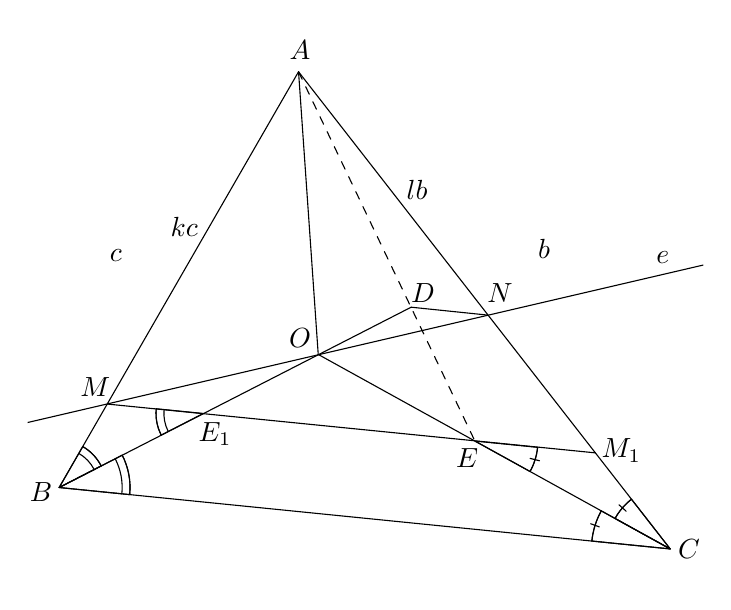
\begin{tikzpicture}[line cap=round,line join=round,>=triangle 45,x=1.0cm,y=1.0cm]
\clip(-3.96,-2.52) rectangle (4.62,4.52);
\draw [shift={(-3.56,-1.32)}] (0,0) -- (27.16:0.6) arc (27.16:60.07:0.6) -- cycle;
\draw [shift={(-1.73,-0.38)}] (0,0) -- (174.26:0.6) arc (174.26:207.16:0.6) -- cycle;
\draw [shift={(-3.56,-1.32)}] (0,0) -- (-5.74:0.9) arc (-5.74:27.16:0.9) -- cycle;
\draw [shift={(4.2,-2.1)}] (0,0) -- (127.91:0.8) arc (127.91:151.09:0.8) -- cycle;
\draw [shift={(1.72,-0.73)}] (0,0) -- (-28.91:0.8) arc (-28.91:-5.74:0.8) -- cycle;
\draw [shift={(4.2,-2.1)}] (0,0) -- (151.09:1) arc (151.09:174.26:1) -- cycle;
\draw (-0.52,3.96)-- (-3.56,-1.32);
\draw (-3.56,-1.32)-- (4.2,-2.1);
\draw (4.2,-2.1)-- (-0.52,3.96);
\draw [domain=-3.96:4.62] plot(\x,{(--0.57--0.31*\x)/1.33});
\draw (-2.95,-0.26)-- (3.25,-0.88);
\draw (0.91,0.97)-- (1.88,0.87);
\draw (0.91,0.97)-- (-3.56,-1.32);
\draw [dash pattern=on 3pt off 3pt] (-0.52,3.96)-- (1.72,-0.73);
\draw (-0.27,0.37)-- (4.2,-2.1);
\draw (-0.52,3.96)-- (-0.27,0.37);
\draw (-2.27,2.24) node[anchor=north west] {$kc$};
\draw (-3.04,1.82) node[anchor=north west] {$c$};
\draw (0.73,2.7) node[anchor=north west] {$lb$};
\draw (2.4,1.96) node[anchor=north west] {$b$};
\draw [shift={(-3.56,-1.32)}] (27.16:0.6) arc (27.16:60.07:0.6);
\draw [shift={(-3.56,-1.32)}] (27.16:0.5) arc (27.16:60.07:0.5);
\draw [shift={(-1.73,-0.38)}] (174.26:0.6) arc (174.26:207.16:0.6);
\draw [shift={(-1.73,-0.38)}] (174.26:0.5) arc (174.26:207.16:0.5);
\draw [shift={(-3.56,-1.32)}] (-5.74:0.9) arc (-5.74:27.16:0.9);
\draw [shift={(-3.56,-1.32)}] (-5.74:0.8) arc (-5.74:27.16:0.8);
\draw [shift={(4.2,-2.1)}] (127.91:0.8) arc (127.91:151.09:0.8);
\draw(3.64,-1.62) -- (3.55,-1.54);
\draw [shift={(1.72,-0.73)}] (-28.91:0.8) arc (-28.91:-5.74:0.8);
\draw(2.42,-0.95) -- (2.54,-0.98);
\draw [shift={(4.2,-2.1)}] (151.09:1) arc (151.09:174.26:1);
\draw(3.3,-1.82) -- (3.19,-1.78);
\draw (3.9,1.8) node[anchor=north west] {$e$};
%\begin{scriptsize}
%\fill [color=black] (-0.52,3.96) circle (1.5pt);
\draw[color=black] (-0.501,4.24) node {$A$};
%\fill [color=black] (-3.56,-1.32) circle (1.5pt);
\draw[color=black] (-3.79,-1.38) node {$B$};
%\fill [color=black] (4.2,-2.1) circle (1.5pt);
\draw[color=black] (4.44,-2.10) node {$C$};
%\fill [color=black] (-0.27,0.37) circle (1.5pt);
\draw[color=black] (-0.5,0.58) node {$O$};
%\fill [color=black] (-2.95,-0.26) circle (1.5pt);
\draw[color=black] (-3.10,-0.05) node {$M$};
%\fill [color=black] (1.88,0.87) circle (1.5pt);
\draw[color=black] (2.04,1.15) node {$N$};
%\fill [color=black] (0.91,0.97) circle (1.5pt);
\draw[color=black] (1.06,1.15) node {$D$};
%\fill [color=black] (1.72,-0.73) circle (1.5pt);
\draw[color=black] (1.62,-0.95) node {$E$};
%\fill [color=black] (3.25,-0.88) circle (1.5pt);
\draw[color=black] (3.58,-0.85) node {$M_1$};
%\fill [color=black] (-1.73,-0.38) circle (1.5pt);
\draw[color=black] (-1.58,-0.64) node {$E_1$};
%\end{scriptsize}
\end{tikzpicture}
\end{center}
\caption*{A 3. feladathoz.}
\end{figure}

Legyen $AM=kc$ és $AN=lb$; hasonlóság szerint $AM_1=kb$, hiszen $BC\parallel MM_1$.

Az $ABC$ háromszög szögfelezője a $B$-nél lévő $\beta$ szöget két egyenlő részre osztja; mivel $BC\parallel MM_1$, így $ME_1B\sphericalangle=\frac{\beta}{2}$. Ezért a $BME_1\triangle$ egyenlő szárú: $MB=ME_1=(1-k)c$. Ezzel megegyező gondolatmenet szerint kapjuk, hogy $M_1C=M_1E=(1-k)b$.

Az $AMN\triangle$-ben felírva a szögfelezőtételt:
\begin{equation}\label{MOON}
\frac{MO}{ON}=\frac{kc}{lb}.
\end{equation}

$DNO\triangle\sim ME_1O\triangle$, mert oldalaik párhuzamosak. A hasonlóságból következően és \eqref{MOON} felhasználásával
\begin{equation}\label{ONOM}
\frac{DN}{ME_1}=\frac{ON}{OM}=\frac{lb}{kc}.
\end{equation}

\eqref{ONOM} szerint
\[\frac{DN}{AN}=\frac{DN}{lb}=\frac{ME_1}{kc}=\frac{1-k}{k}.\]

De $\frac{EM_1}{AM_1}=\frac{1-k}{k}$, ezért pedig $ADN\triangle\sim AEM_1\triangle$, mert két oldaluk aránya és (a párhuzamosság miatt) egy szögük megegyezik.

Ezért az $A$ csúcsnál lévő szögük is megegyezik, tehát $A$, $D$ és $E$ kollineárisak.

\medskip

\vonal
{\bf 4. feladat: } 
Az $ABC$ háromszög $A$ csúcsához tartozó magasságának a $BC$ oldal egyenesén levő talppontja $D$. A $B$ és $C$ pontokból az $A$ csúcsból induló belső szögfelezőre bocsátott merőlegesek talppontjai rendre $E$ és $F$. Az $EF$ és $BC$ szakaszok metszéspontja $M$. Legyen az $ABC$ háromszög területe $T$, a $DEF$ háromszög területe $t$.

Bizonyítsuk be, hogy
\[\sqrt{\frac t T} = \frac{FM \cdot BM \cdot DE}{EM \cdot CM \cdot AB}.\]

\ki{Bíró Bálint}{Eger}\medskip

{\bf Megoldás: } A feltételeknek megfelelő ábrát készítünk.

Az $AB$ szakasz a $D$ és $E$ pontokból derékszögben látszik, ezért $D$ és $E$ rajta van az $AB$ mint átmérő fölé írt Thalész-körön. Ebből az is következik, hogy $ABED$ húrnégyszög.
Hasonlóképpen mivel az $AC$ szakasz a $D$ és $F$ pontokból derékszögben látszik, ezért $D$
és $F$ illeszkedik az $AC$ Thalész-körére, és ezért $ACDF$ húrnégyszög.

Mivel $ABED$ húrnégyszög, ezért $DEF\sphericalangle = DEA\sphericalangle = DBA\sphericalangle$, mert az utóbbi két szög az $AD$ húrhoz tartozó kerületi szög. $ACDF$ is húrnégyszög, amelynek szemben fekvő szögei 180\degre-ra egészítik ki egymást, azaz $ACD\sphericalangle+ DFA\sphericalangle = 180\degre$.

\begin{figure}
\begin{center}
\definecolor{qqwwzz}{rgb}{0,0.4,0.6}
\definecolor{ubqqys}{rgb}{0.29,0,0.51}
\definecolor{ttzzqq}{rgb}{0.2,0.6,0} % szép zöld a körökhöz, végül nem használva
\begin{tikzpicture}[line cap=round,line join=round,>=triangle 45,x=1.2cm,y=1.2cm]
\clip(-4.76,-1.5) rectangle (3.56,4.1);
\draw [shift={(-0.64,1.46)}] (0,0) -- (122.03:0.3) arc (122.03:212.03:0.3) -- cycle;
\draw [shift={(0.95,2.46)}] (0,0) -- (-147.97:0.3) arc (-147.97:-57.97:0.3) -- cycle;
\draw [shift={(-0.8,2.52)}] (0,0) -- (138.25:0.3) arc (138.25:228.25:0.3) -- cycle;
\draw [shift={(-3.14,-0.1)}] (0,0) -- (-7.69:0.8) arc (-7.69:32.03:0.8) -- cycle;
\draw [shift={(-0.8,2.52)}] (0,0) -- (-41.75:0.6) arc (-41.75:-2.02:0.6) -- cycle;
\draw [shift={(-3.14,-0.1)}] (0,0) -- (32.03:0.6) arc (32.03:71.75:0.6) -- cycle;
\fill[color=ubqqys,fill=ubqqys,fill opacity=0.25] (-0.8,2.52) -- (-0.64,1.46) -- (0.95,2.46) -- cycle;
\fill[color=qqwwzz,fill=qqwwzz,fill opacity=0.2] (-1.94,3.54) -- (-3.14,-0.1) -- (3.08,-0.94) -- cycle;
\draw (-3.14,-0.1)-- (3.08,-0.94);
\draw (3.08,-0.94)-- (-1.94,3.54);
\draw (-1.94,3.54)-- (-3.14,-0.1);
\draw (-0.8,2.52)-- (-3.14,-0.1);
\draw [domain=-4.76:3.56] plot(\x,{(--1.58--0.53*\x)/0.85});
\draw (-0.8,2.52)-- (-0.64,1.46);
\draw (-0.8,2.52)-- (0.95,2.46);
\draw [color=black] (-0.03,-0.52) circle (3.7659cm);
\draw [color=black] (-2.54,1.72) circle (2.2996cm);
\draw (0.95,2.46)-- (3.08,-0.94);
\draw (-1.94,3.54)-- (-0.64,1.46);
\fill(-0.81,1.5) circle (0.02);
\fill(0.91,2.29) circle (0.02);
\fill(-0.98,2.51) circle (0.02);
\draw [shift={(-3.14,-0.1)}] (-7.69:0.8) arc (-7.69:32.03:0.8);
\draw [shift={(-3.14,-0.1)}] (-7.69:0.7) arc (-7.69:32.03:0.7);
\draw [shift={(-0.8,2.52)}] (-41.75:0.6) arc (-41.75:-2.02:0.6);
\draw [shift={(-0.8,2.52)}] (-41.75:0.5) arc (-41.75:-2.02:0.5);
\draw [shift={(-3.14,-0.1)}] (32.03:0.6) arc (32.03:71.75:0.6);
\draw [shift={(-3.14,-0.1)}] (32.03:0.5) arc (32.03:71.75:0.5);
%\begin{scriptsize}
%\fill [color=black] (-3.14,-0.1) circle (1.5pt);
\draw[color=black] (-3.3,0.15) node {$A$};
%\fill [color=black] (3.08,-0.94) circle (1.5pt);
\draw[color=black] (3.30,-0.96) node {$B$};
%\fill [color=black] (-1.94,3.54) circle (1.5pt);
\draw[color=black] (-1.93,3.73) node {$C$};
%\fill [color=black] (-0.8,2.52) circle (1.5pt);
\draw[color=black] (-0.64,2.7) node {$D$};
%\fill [color=black] (0.95,2.46) circle (1.5pt);
\draw[color=black] (0.97,2.65) node {$E$};
%\fill [color=black] (-0.64,1.46) circle (1.5pt);
\draw[color=black] (-0.55,1.3) node {$F$};
%\fill [color=black] (-0.04,1.84) circle (1.5pt);
\draw[color=black] (0.27,1.82) node {$M$};
%\end{scriptsize}
\end{tikzpicture}
\end{center}
\caption*{A 4. feladathoz.}
\end{figure}

A $DFA\sphericalangle$ és $DFE\sphericalangle$ szögek ugyancsak 180\degre-ra egészítik ki egymást, így $ACD\sphericalangle = ACB\sphericalangle = DFE\sphericalangle$.

A $DEF$ és $ABC$ háromszögekben tehát két-két szög, mégpedig a $DEF\sphericalangle = CBA\sphericalangle$ és a $DFE\sphericalangle = ACB\sphericalangle$ szögek nagysága egyenlő, ezért a harmadik szögek mértéke is azonos, vagyis a két háromszög hasonló: $DEF\triangle\sim ABC\triangle$.

Hasonló háromszögek területének aránya a hasonlóság arányának négyzetével egyenlő, ezért
\[\frac t T = \left(\frac{FD}{AC}\right)^2,\]
ebből pedig
\[\sqrt{\frac t T}=\frac{FD}{AC}\]
következik.

A $DEF$ és $ABC$ háromszögekben tehát $EDF\sphericalangle = BAC\sphericalangle$.

Viszont az $ABED$ húrnégyszögben az $EDB\sphericalangle$ és az $EAB\sphericalangle$ azonos íven nyugvó kerületi szögek, tehát egyenlők. A feltétel szerint az $AE$ egyenese felezi a $BAC\sphericalangle$-et, így 
\[EAB\sphericalangle=\frac{BAC\sphericalangle}{2}=\frac{EDF\sphericalangle}{2}=EDB\sphericalangle,\]
ez pedig éppen azt jelenti, hogy a $BC$ egyenes felezi az $EDF$ szöget.

Felírjuk a szögfelezőtételt az $ABC\triangle$-ben:
\begin{equation}\label{AC}
\frac{AC}{AB}=\frac{CM}{BM}\implies AC=\frac{AB\cdot CM}{BM}.
\end{equation}

A $DEF\triangle$-ben is felírjuk a szögfelezőtételt:
\begin{equation}\label{FD}
\frac{FD}{DE}=\frac{FM}{EM}\implies FD=\frac{DE\cdot FM}{EM}.
\end{equation}

\eqref{AC} és \eqref{FD} eredményét a $\sqrt{\frac{t}{T}}$-re vonatkozó képletbe való beírásával kapjuk a bizonyítandó állítást:
\[\sqrt{\frac t T}=\frac{FD}{AC}=\frac{FM \cdot BM \cdot DE}{EM \cdot CM \cdot AB}.\]

\medskip

\vonal
{\bf 5. feladat: } 
Adott egy tetszőleges poliéder. Lehet-e a csúcsaiba pozitív egész számokat írni a következő módon:
\begin{itemize}
\item[] 
ha él köt össze két csúcsot, akkor a csúcsokba írt számok relatív prímek;
\item[] 
ha két csúcs nincs éllel összekötve, akkor a csúcsokba írt számok legnagyobb közös osztója 1-nél nagyobb?
\end{itemize}

\ki{Kántor Sándor}{Debrecen}\medskip

{\bf Megoldás: } Az elhelyezés lehetséges, ennek bizonyítását egy, a feltételeknek megfelelő elhelyezés megadásával végezzük. Az elhelyezés során számokat fogunk írni a csúcsokba és a végső értéket a beírt számok szorzata fogja jelenteni.

Először vegyük a csúcsokat valamilyen sorrendben és az első csúcsra írjuk az első prímszámot (2-t), a második csúcsra a második prímszámot (3-at), és így tovább a többi csúcsra. Ez véges sok lépés után véget ér.

Ezek után vegyük az első olyan párt, amelyiket nem köt össze él és mindkét csúcsba írt aktuális számot szorozzuk meg a soron következő prímszámmal. Majd vegyük a következő össze nem kötött párt, és folytassuk ezt az eljárást. Ez is véges sok lépés után véget ér.

A feltételek teljesülnek:
\begin{itemize}
\item Ha él köt össze két csúcsot, akkor azokban csupa különböző prímszámot szoroztunk össze, hiszen közös prímosztó csak akkor kerülhetne mind a kettőbe, ha nem lennének összekötve.
\item Ha nem köt össze él két csúcsot, akkor van olyan prím, ami mind a kettőben szerepel, tehát a legnagyobb közös osztójuk biztosan nem 1.
\end{itemize}

Tehát ez az elhelyezés kielégíti a feltételeket.
\medskip

\vonal
{\bf 6. feladat: } 
Létezik-e olyan négyzetszám, amelynek a számjegyeinek összege  $2011^{2010}$?

\ki{Szabó Magda}{Szabadka}

{\bf I. megoldás: } Megmutatjuk, hogy létezik olyan szám.

Tekintsük az $x=2\cdot10^k-1$ alakú számokat, ahol $k$ pozitív egész szám.
\begin{align*}
x^2&=\left(2\cdot10^k-1\right)^2=4\cdot10^{2k}-4\cdot10^k+1\\
&=4\underbrace{00\ldots0}_{2k}-4\underbrace{00\ldots0}_{k}+1=3\underbrace{99\ldots9}_{k-1}6\underbrace{00\ldots0}_{k-1}1
\end{align*}
Eszerint $x^2$ számjegyeinek összege $3+(k-1)\cdot9+6+1=9k+1$.

Ha $k$ értékét egyesével növeljük, akkor a számjegyek összege minden lépésben 9-cel fog nőni, ezért minden $9n+1$ alakú értéket fel fog venni.

Most megmutatjuk, hogy $2011^{2010}\equiv1\pmod{9}$, azaz $x^2$ számjegyeinek összege ezt az értéket is felveszi.
\[2011^3\equiv4^3\equiv64\equiv1\pmod9\]
\[2011^{2010}\equiv\left(2011^3\right)^{670}\equiv1^{670}\equiv1\pmod9\]
Tehát $2011^{2010}$ valóban $9n+1$ alakú szám, így $x^2$ számjegyeinek összege ennyi lesz valamely $k$-ra.

\medskip

{\bf II. megoldás: } Tekintsük az
\[y=\underbrace{33\ldots3}_{k-1}2=\frac{10^k-4}{3}\]
számokat, ahol $k$ pozitív egész szám. Ekkor
\begin{align*}
y^2&=\underbrace{33\ldots3}_{k-1}2^2=\left(\frac{10^k-4}{3}\right)^2=\frac19\left(10^{2k}-8\cdot10^k+16\right)\\
&=\frac19\left(10^{2k}\right)-8\cdot\frac19\left(10^k-1\right)+1=\underbrace{11\ldots1}_{2k}-\underbrace{88\ldots8}_k+1\\
&=\underbrace{11\ldots1}_{k-1}0\underbrace{22\ldots2}_{k-1}4
\end{align*}
Így $y^2$ számjegyeinek összege $(k-1)\cdot1+0+(k-1)\cdot2+4=3k+1$.

Ha $k$ értékét egyesével növeljük, akkor a számjegyek összege minden lépésben 3-mal fog nőni, tehát minden $3n+1$ alakú értéket fel fog venni. $2011^{2010}$-ről pedig az \textit{I.~megoldás} végén megmutattuk, hogy $9n+1$ alakú szám, tehát $3n+1$ alakú szám is.

Így $y^2$ számjegyeinek összege valamely $k$-ra $2011^{2010}$ lesz.

\end{document}